\chapter{Modeling Using Usecases}\label{chapter:selection_by_use_case}
\section{Use case}\label{section:selection_by_use_case/use_case}
A use case is an efficient as well as a fancy way of capturing requirements. Another technique of eliciting requirement is by features specification. However, the feature specification technique limits itself to answer only "what the system is intended to do". On the other hand, use case goes further and specifies "what the system does for any specific kind of user". In this way, it gives a way to specify and most importantly validate the expectation and concerns of stakeholders at the very early phase of software development. Undoubtedly for the same reason, it is not just a tool for requirement specification but an important software engineering technique which guides the software engineering cycle. Using use cases, the software can be developed to focus on the concerns that are valueable to the stakeholders and test accordingly.\cite{Ng:2004aa}
\\
It can be valueable to see the ways it has been defined.
\begin{shaded}Definition 1: \cite{Jacobson:1987aa} \end{shaded}
"A use case is a sequence of actions performed by the system to yield an observable result of value to a particular user." 
\\
\begin{shaded}Definition 2: \cite{Rumbaugh:1999aa}\end{shaded}
"A use case is a description of a set of sequences of actions, including variants, that a system performs that yield an observable result of value to an actor."

\section{Use case Refactoring}\label{section:selection_by_use_case/use_case_refactoring}
According to \cite{Jacobson:1987aa} it is not always intuitive to modularize use cases directly. As per the definitions provided in \ref{section:selection_by_use_case/use_case}, a use case consists of a number of ordered functions together to accomplish a certain goal. \cite{Jacobson:1987aa} defines these cohesive functionalites distributed across usecases as clusters. And the process of identifying the clusters scattered around the use cases is the process of identifying services. \cite{Ng:2004aa} and \cite{Jacobson:2003aa} describes use case possibly consisting of various cross-cutting concerns. The papers use the term 'use case module' to define the cohesive set of tasks. The figure \ref{fig:selection_by_use_case/use_case_one} demonstrate the cross cutting functionalities needed by a use case in order to accomplish its goal. For example, the use case 'does A' has to perform separate functionalities on different domain entities X and Y. Similarly, the use case 'does B' needs to perform distinct functions on entities X, Y and Z.
\begin{figure}[H]
\begin{center}
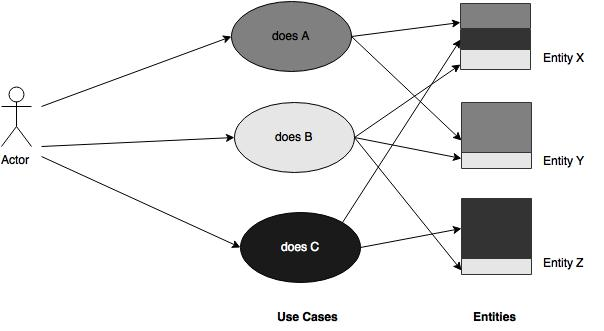
\includegraphics[width=0.8\textwidth]{figures/use-case-one}
\caption{Use cases with cross-cutting concerns \cite{Ng:2004aa}}
\label{fig:selection_by_use_case/use_case_one}
\end{center}
\end{figure}
This situation prompts for the analysis of the use cases for cross cutting tasks and refactoring them in order to map the cohesive functionalities and use cases. Refactoring helps to achieve the right level of abstraction and granularity by improving functionality cohesion as well as elimination of redundancy and finally promoting the reusablity. \cite{Doh:2007aa}
\\
Furthermore, the refactoring is assisted by various relationships in use case model to represent dependencies between use cases, which are include, generalization and extend. \cite{Ng:2004aa}
\\
\section{Process for Use Case Refactoring}\label{section:selection_by_use_case/process_for_use_case_refactoring}
In order to refactor the use cases and finally map use cases to the service, the papers \cite{Kim:2006aa}, \cite{Yun:2006aa} and \cite{Doh:2007aa} provide a comprehensive method. It is a type of meet-in-the-middle approach where use case models are first created and then refactored to create new set of use cases to accomplish high cohesion in functionality and loose coupling. This will ultimately create use cases supporting modularity and autonomy. \cite{Fareghzadeh:2008aa} There are three distinct steps for service identification using service refactoring.
\begin{enumerate}
\item \textbf{TaskTree Generation}\\
In this step, the initial use case model created during domain analysis is used to create task trees for each distinct use case. The task trees provide sequence of individual tasks required to accomplish in order to achieve the goal of the use case.
\\
\item \textbf{Use Case Refactoring}\\
In this step, the task tree generated in the previous step is analysed. As already mentioned in the section \ref{section:selection_by_use_case/use_case_refactoring}, that the initial use case consists of various cross cutting functionalities which runs through large number of business entities. In order to minimize that, refactoring is performed. The detail rules are provided in section \ref{section:selection_by_use_case/rules_for_use_case_refactoring}.
\\
\item \textbf{Service Identification}\\
The use cases achieved after refactoring have correct level of abstractions and granularity representing cohesive business functionality. The unit use cases thus achieved appreciate reuse of common functionality.  \cite{Doh:2007aa} Furthermore, the approach considers the concerns of stakeholders in terms of cohesive business functionalities to be represented by use cases.\cite{Fareghzadeh:2008aa} Additionally, the process also clarifies the dependencies between various use cases. Thus, the final use cases obtained can be directly maped to individual services.
\end{enumerate}
\\
\section{Rules for Use Case Refactoring}\label{section:selection_by_use_case/rules_for_use_case_refactoring}
The context is first defined before distinct rules are presented.
\\
\begin{shaded}Context 1 \end{shaded}
If U represents use case model of the application, $t_i$ represents any task of U and T being the set of tasks of U. Then, $\forall t_i \in T $, $t_i$ exists in the post-refactoring model U'. The refactoring of a use case model preserves the set of tasks.
\\
\begin{shaded}Context 2 \end{shaded}
A refactoring rule R is defined as a 3-tuple (Parameters, Preconditions, Postconditions). Parameters are the entities involved in the refactoring, precondition defines the condition which must be satisfied by the usecase u in order for R to be applied in u. Postcondition defines the state of U after R is applied.
\\
The various refactoring rules are as listed below.
\\
\subsection{Decomposition Refactoring}\label{section:selection_by_use_case/guidelines_for_use_case_refactoring/decomposition_refactoring}
When the usecase is complex and composed of various functionally independent tasks, the tasks can be ejected out of the task tree of the usecase and represented as a new use case. The table \ref{tab:selection_by_use_case/guidelines_for_use_case_refactoring/decomposition_rule} shows the decomposition rule in detail.
\begin{table}[H]
  \centering
  \begin{adjustbox}{max width=\textwidth}
  \begin{tabular}{*{14}{|c}|}%%{|c|l|}
  \hline
  Parameters & 
                    \begin{tabular}{ll}
                    \multirow{3}{*}
                    &u: a use case to be decomposed\\
                    &t: represents task tree of u \\
                    &t': a subtask tree of t\\
                    \end{tabular}\\
                    \hline
   Preconditions  & t' is functionally independent of u \\
                    \hline
   Postconditions &
                    \begin{tabular}{ll}
                    \multirow{2}{*}
                    &1. new use case u' containing task tree t' is generated \\
                    &2. a dependency is created between u and u'\\
                    \end{tabular}\\
                    \hline
\end{tabular}
\end{adjustbox}
  \caption{Decomposition Rule}
  \label{tab:selection_by_use_case/guidelines_for_use_case_refactoring/decomposition_rule}
\end{table}
\\

\subsection{Equivalence Refactoring}\label{section:selection_by_use_case/guidelines_for_use_case_refactoring/equivalence_refactoring}
If the two use cases share their tasks in the task tree, we can conclude that they are equivalent and redundant in the use case model. The table \ref{tab:selection_by_use_case/guidelines_for_use_case_refactoring/equivalence_rule} shows the rule for the refactoring.
\begin{table}[H]
  \centering
  \begin{adjustbox}{max width=\textwidth}
  \begin{tabular}{*{14}{|c}|}%%{|c|l|}
  \hline
  Parameters &  $u_1$ , $u_2$: two distinct use cases\\
                    \hline
   Preconditions  & the task trees of $u_1$ and $u_2$ have same behavior \\
                    \hline
   Postconditions &
                    \begin{tabular}{ll}
                    \multirow{3}{*}
                    &1. $u_2$ is replaced by $u_1$ \\
                    &2. all the relationship of $u_2$ are fulfilled by $u_1$\\
                    &3. $u_2$ has no relationship with any other use cases\\
                    \end{tabular}\\
                    \hline
\end{tabular}
\end{adjustbox}
  \caption{Equivalence Rule}
  \label{tab:selection_by_use_case/guidelines_for_use_case_refactoring/equivalence_rule}
\end{table}
\\

\subsection{Composition Refactoring}\label{section:selection_by_use_case/guidelines_for_use_case_refactoring/composition_refactoring}
When there are two or more small-grained use cases such that they have related tasks, the use cases can be represented by a composite unit use case.

\begin{table}[H]
  \centering
  \begin{adjustbox}{max width=\textwidth}
  \begin{tabular}{*{14}{|c}|}%%{|c|l|}
  \hline
  Parameters & 
                 \begin{tabular}{ll}
                    \multirow{3}{*}
                    & $u_1$, $u_2$: the fine grained use cases\\
                    & $t_1$, $t_2$: the task trees of $u_1$ and $u_2$ respectively\\
                    \end{tabular}\\
                    \hline
   Precondition     & $t_1$ and $t_2$ are functionally related.\\
                    \hline
   Postconditions &
                    \begin{tabular}{ll}
                    \multirow{3}{*}
                    & 1. $u_1$ and $u_2$ are merged to a new unit use case u \\
                    & 2. u has new task tree given by $t_1 \cup t_2 $\\
                    & 3. the dependencies of $u_1$ and $u_2$ are handled by u\\ 
                    & 4. $u_1$ and $u_2$ are deleted along with their task trees $t_1$ and $t_2$\\
                    \end{tabular}\\
                    \hline
\end{tabular}
\end{adjustbox}
  \caption{Composition Rule}
  \label{tab:selection_by_use_case/guidelines_for_use_case_refactoring/composition_rule}
\end{table}
\\

\subsection{Generalization Refactoring}\label{section:selection_by_use_case/guidelines_for_use_case_refactoring/generalization_refactoring}
When multiple use cases share some volume of dependent set of tasks in their task trees, it can be implied that the common tasks set can be represented by a new use case. The table \ref{tab:selection_by_use_case/guidelines_for_use_case_refactoring/generalization_rule} provides the specific of the rule.
\begin{table}[H]
  \centering
  \begin{adjustbox}{max width=\textwidth}
  \begin{tabular}{*{14}{|c}|}%%{|c|l|}
  \hline
  Parameters & 
                 \begin{tabular}{ll}
                    \multirow{2}{*}
                    & $u_1$ , $u_2$: two distinct use cases\\
                    & $t_1$ , $t_2$: task trees of $u_1$ and $u_2$ respectively\\
                    \end{tabular}\\
                    \hline
   Precondition     & $t_1$ and $t_2$ share a common set of task $t= \{ x_1, x_2...x_n \} $\\
                    \hline
   Postconditions &
                    \begin{tabular}{ll}
                    \multirow{5}{*}
                    & 1. a new use case u is created using task tree $t= \{x_1, x_2...x_n \} $ \\
                    & 2. relationship between u with $u_1$  and between u with $u_2$ is created\\
                    & 3. the task tree $t= \{ x_1, x_2...x_n \} $ is removed from task tree of both $u_1$ and $u_2$\\
                    & 4. the common relationship of both $u_1$ and $u_2$ are handled by u and \\ 
                    & removed from them\\
                    \end{tabular}\\
                    \hline
\end{tabular}
\end{adjustbox}
  \caption{Generalization Rule}
  \label{tab:selection_by_use_case/guidelines_for_use_case_refactoring/generalization_rule}
\end{table}
\\


\subsection{Merge Refactoring}\label{section:selection_by_use_case/guidelines_for_use_case_refactoring/merge_refactoring}
When a use case is just specific for another use case and the use case is only the consumer for it, the two use cases can be merged into one.
\begin{table}[H]
  \centering
  \begin{adjustbox}{max width=\textwidth}
  \begin{tabular}{*{14}{|c}|}%%{|c|l|}
  \hline
  Parameters & 
                 \begin{tabular}{ll}
                    \multirow{3}{*}
                    & u, u': the use cases\\
                    & r defines the dependency of u with u'\\
                    & t, t': the task trees of u and u' respectively\\
                    \end{tabular}\\
                    \hline
   Precondition     & there is no dependency of other usecases with u' except u\\
                    \hline
   Postconditions &
                    \begin{tabular}{ll}
                    \multirow{3}{*}
                    & 1. u' is merged to u \\
                    & 2. u has new task tree given by $t \cup t' $\\
                    & 3. r is removed\\
                    \end{tabular}\\
                    \hline
\end{tabular}
\end{adjustbox}
  \caption{Merge Rule}
  \label{tab:selection_by_use_case/guidelines_for_use_case_refactoring/merge_rule}
\end{table}
\\

\subsection{Deletion Refactoring}\label{section:selection_by_use_case/guidelines_for_use_case_refactoring/deletion_refactoring}
When a use case is defined but no relationship can be agreed with other use cases or actors then it can be referred that the use case represent redundant set of tasks which has already been defined by other use cases.
\begin{table}[H]
  \centering
  \begin{adjustbox}{max width=\textwidth}
  \begin{tabular}{*{14}{|c}|}%%{|c|l|}
  \hline
  Parameters      & u: a distinct use case\\
                    \hline
   Precondition     & the use case u has no relationship with any other usecases and actors\\
                    \hline
   Postconditions   & the use case u is deleted\\
                    \hline
\end{tabular}
\end{adjustbox}
  \caption{Deletion Rule}
  \label{tab:selection_by_use_case/guidelines_for_use_case_refactoring/deletion_rule}
\end{table}
\\

\section{Example Scenario}\label{section:selection_by_use_case/refactoring_example}
In this section, a case study will be taken as an example. The case study will be modeled using use case. Finally, the use case will be refactored using the rules given by \ref{section:selection_by_use_case/guidelines_for_use_case_refactoring}.
\\
\begin{shaded} Case Study \end{shaded}
The case study is about an international hotel named 'XYZ' which has branches in various locations. In each location, it offers rooms with varying facilities as well as prices. In order to make it easy for customers to find room irrespective of the location of customer, it is planning to offer an online room booking application. Using this application, any registered customer can search for a room according to his/her requirement in any location. When he/she is satisfied, can book the room online as well. The customer will be sent notification by email regarding booking. At present, the payment will be accepted in person, only after the customer gets into the respective branch. Finally, if the customer wants to cancel the room, he/she can do online anytime. The customer will also be notified by e-mail to confirm the cancelation of booking. It is an initial case study so only priority cases and conditions are considered here.
\\
\\
The remaining part of this section presents the steps to indentify the services using use case refactoring following the process defined in section \ref{section:selection_by_use_case/process_for_use_case_refactoring} and rules presented in the section \ref{section:selection_by_use_case/rules_for_use_case_refactoring}
\\
\\
\textbf{\underline{Step 1:}}
\\
\\
The initial analysis of the case study will produce use case model as given by figure \ref{fig:selection_by_use_case/use_case_two}.

\begin{figure}[H]
\begin{center}
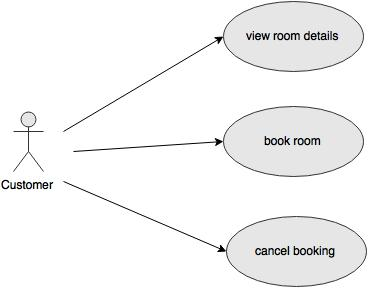
\includegraphics[width=0.8\textwidth]{figures/use-case-two}
\caption{Initial Use Case Model for Online Room Booking Application}
\label{fig:selection_by_use_case/use_case_two}
\end{center}
\end{figure}
\\
\\
\textbf{\underline{Step 2:}}
\\
\\
For each initial use case, task trees are generated which are needed to accomplish the desired functionality of respective use cases.
\\
\begin{table}[H]
  \centering
  \begin{adjustbox}{max width=\textwidth}
  \begin{tabular}{*{14}{|c}|}%%{|c|l|}
  \hline
  \textbf{Use Case} & \textbf{Task Tree} \\
  \hline
  book room & 
                 \begin{tabular}{ll}
                    \multirow{9}{*}
                    & customer enters access credentials\\
                    & system validates the credentials\\
                    & customer enters location and time details for booking\\
                    & system fetch the details of empty rooms according to the data provided\\
                    & system displays the details in muliple pages\\
                    & customer choose the room and submits for booking\\
                    & system generates a booking number\\
                    & System updates the room\\
                    & system sends notification to the customer regarding booking\\
                    \end{tabular}\\
                    \hline
   cancel booking   &
                    \begin{tabular}{ll}
                    \multirow{7}{*}
                    & customer enters access credentials\\
                    & system validates the credentials\\
                    & customer enters the booking number\\
                    & system validates the booking number\\
                    & customer cancels the booking\\
                    & system updates the room\\
                    & system sends notification to the customer regarding cancelation\\
                    \end{tabular}\\
                    \hline
   view room details &
                    \begin{tabular}{ll}
                    \multirow{5}{*}
                    & customer enters access credentials\\
                    & system validate the credentials\\
                    & customer enter location and time\\
                    & system fetch the details of empty rooms according to the data provided\\
                    & system display the details in multiple pages\\
                    \end{tabular}\\
                    \hline
\end{tabular}
\end{adjustbox}
  \caption{Task Trees for Initial Use Cases}
  \label{tab:selection_by_use_case/guidelines_for_use_case_refactoring/initial_task_tree}
\end{table}
\\
\textbf{\underline{Step 3:}}
\\
The initial task trees created for each use case at Step 2 is analysed. There are quite a few set of tasks which are functionally independent of the use case goal and also few tasks which are common in more use use cases. The following table \ref{tab:selection_by_use_case/guidelines_for_use_case_refactoring/common_and_independent_tasks} lists those tasks from the tasks trees \ref{tab:selection_by_use_case/guidelines_for_use_case_refactoring/initial_task_tree} which are either functionally independent from their corresponding use cases or common in more use cases.
\\
\begin{table}[H]
  \centering
  \begin{adjustbox}{max width=\textwidth}
  \begin{tabular}{*{14}{|c}|}%%{|c|l|}
  \hline
  \textbf{Tasks Type} & \textbf{Tasks} \\
  \hline
  Independent Tasks & 
                 \begin{tabular}{ll}
                    \multirow{9}{*}
                    & system validates the credentials\\
                    & system fetch the details of empty rooms according to the data provided\\
                    & system generates a booking number\\
                    & system validates the booking number\\
                    & system updates the room\\
                    & system sends notification to the customer
                    \end{tabular}\\
                    \hline
   Common Tasks   &
                \begin{tabular}{ll}
                    \multirow{9}{*}
                    & system validates the credentials\\
                    & system fetch the details of empty rooms according to the data provided\\
                    & system updates the room\\
                    & system sends notification to the customer
                    \end{tabular}\\
                    \hline
\end{tabular}
\end{adjustbox}
  \caption{Common and Independent Tasks}
  \label{tab:selection_by_use_case/guidelines_for_use_case_refactoring/common_and_independent_tasks}
\end{table}
\\
Now, for independent tasks the docomposition rule given by \ref{tab:selection_by_use_case/guidelines_for_use_case_refactoring/decomposition_rule} can be applied and for common tasks, the generalization rule given by \ref{tab:selection_by_use_case/guidelines_for_use_case_refactoring/generalization_rule} can be applied. The use cases obtained after applying these rules is shown by the figure \ref{fig:selection_by_use_case/use_case_three}
\\
\begin{figure}[H]
\begin{center}
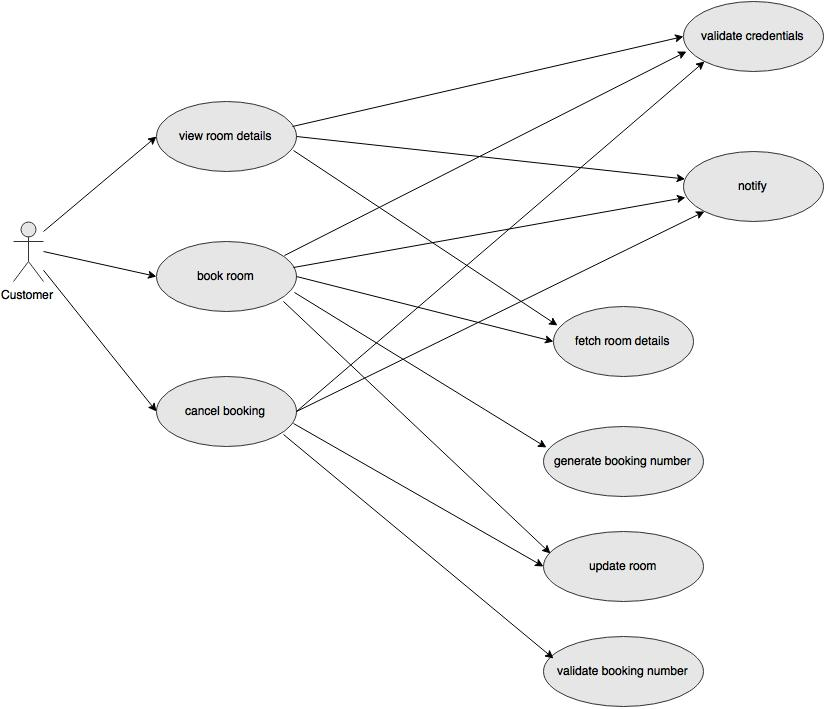
\includegraphics[width=0.8\textwidth]{figures/use-case-three}
\caption{Use Case Model after applying Decomposition and Generalization rules}
\label{fig:selection_by_use_case/use_case_three}
\end{center}
\end{figure}
\\
\textbf{\underline{Step 4:}}
\\
The use case model \ref{fig:selection_by_use_case/use_case_three} obtained in Step 3 is analysed again for further refactoring. It can seen that the use cases 'fetch room details' and 'update room' are fine grained and related to same business model 'Room'. Similarly, the use cases 'generate booking number' and 'validate booking number' are related to business entity 'Booking Number'. The composition rule given by \ref{tab:selection_by_use_case/guidelines_for_use_case_refactoring/composition_rule} can be applied to these use cases, which will then result in use case model given by figure \ref{fig:selection_by_use_case/use_case_four}
\\
\begin{figure}[H]
\begin{center}
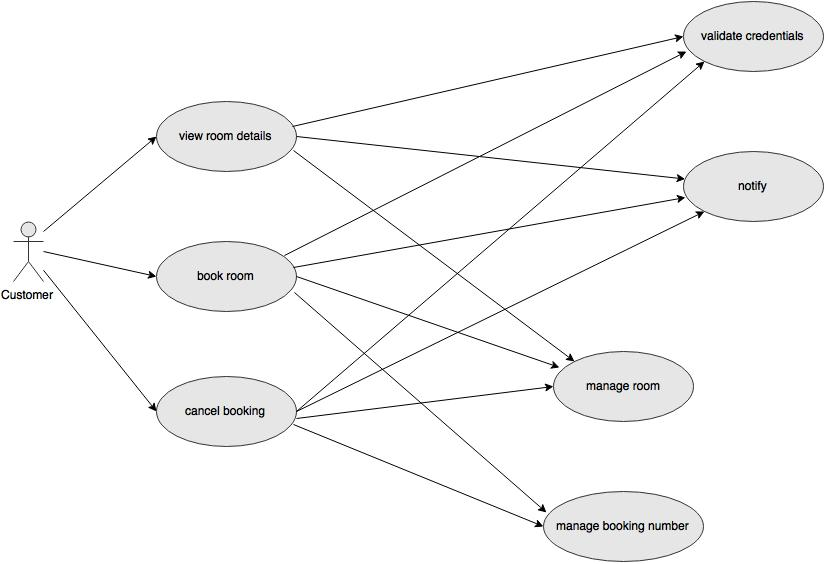
\includegraphics[width=0.8\textwidth]{figures/use-case-four}
\caption{Use Case Model after applying Composition rule}
\label{fig:selection_by_use_case/use_case_four}
\end{center}
\end{figure}
\\
\textbf{\underline{Step 5:}}
\\
Finally, the use case obtained in step 4 is used to identify the service candidates. The final use cases obtained in Step 4 have appropriate level of granularity and cohesive functionalities to be identified as individual services. Most importantly, the refactoring has now separated the cross cutting concerns in terms of various reusable fine grained use cases as shown by the figure. If we compare the the final use case model \ref{fig:selection_by_use_case/use_case_five} with respect to figure \ref{fig:selection_by_use_case/use_case_one}, then it can be implied that the functionalities operating on business entities as well as the business logic serving the candidate concerns are separated and represented by individual use cases. So, the each use case can be mapped to individual services. The services are as listed in the bottom of the figure \ref{fig:selection_by_use_case/use_case_five}.
\\
\begin{figure}[H]
\begin{center}
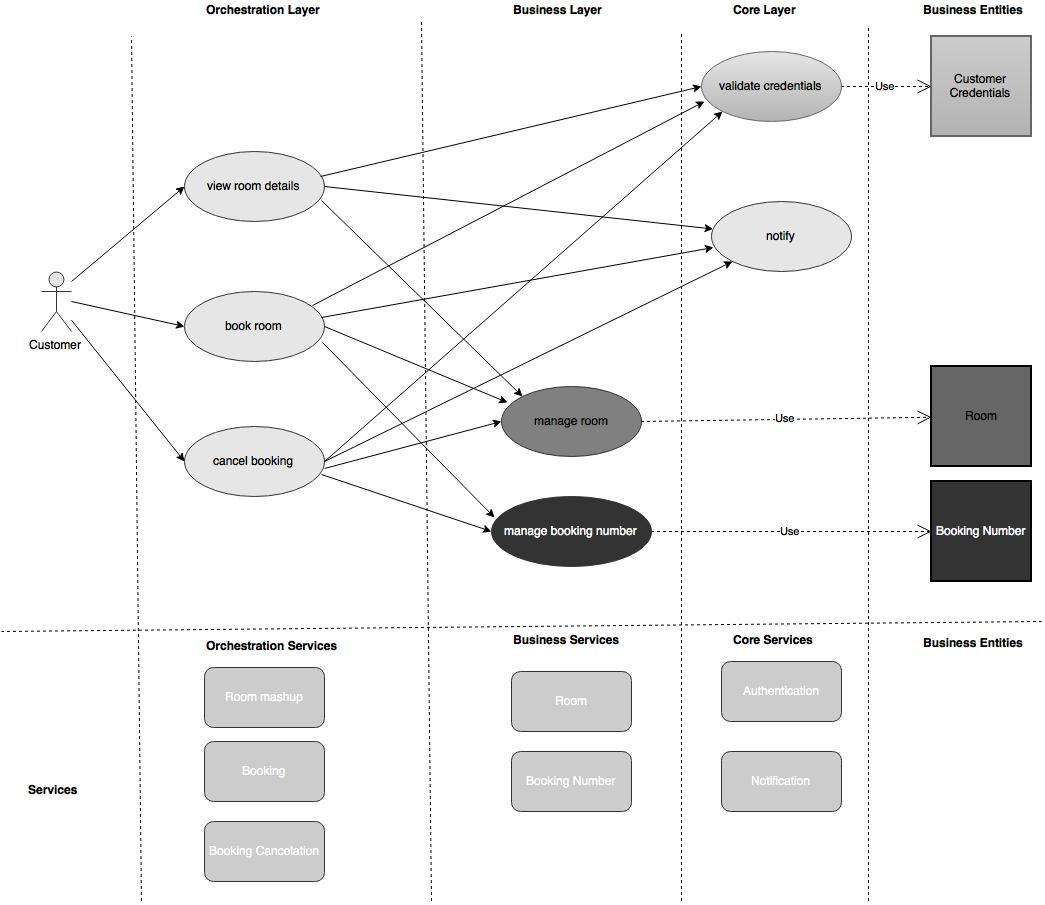
\includegraphics[width=0.8\textwidth]{figures/use-case-five}
\caption{Use Case Model for identification of service candidates}
\label{fig:selection_by_use_case/use_case_five}
\end{center}
\end{figure}
\\
\textbf{Service Layers}\\
The services or use cases obtained from the refactoring creates various levels of abstractions. The levels of abstractions represents different level of functionality. The services at the bottom layer are core services which serve many higher level services. These services are not dependent on any other services. 'Notification' and 'Authentication' are core services obtained from refactoring. The layer above the core layer is business layer. The business service can either have entity services, which control some related business entities or can have task services which provides some specific business logic to higher level services. 'Room' and 'Booking Number' are the entity services obtained from refactoring. Finally, the top layer is mashup layer which contains high level business logic and collaborates with business services as well as core services. 'Room mashup' , 'Booking' and 'Booking Cancelation' are orchestration layer services obtained. The individual services as well as their respective layers are given in figure \ref{fig:selection_by_use_case/use_case_five}. \cite{Fareghzadeh:2008aa}\cite{Emig:2015aa}\cite{Zimmermann:2005aa}
